\documentclass{article}
\usepackage{graphicx}


\begin{document}

\title {Exposure Time Calculator: code and algorithm}
\author{David Kirkby \& An\v{z}e Slosar}
\date{Version 0.1}
\maketitle

\section{Algorithms}

\begin{figure}\centering
  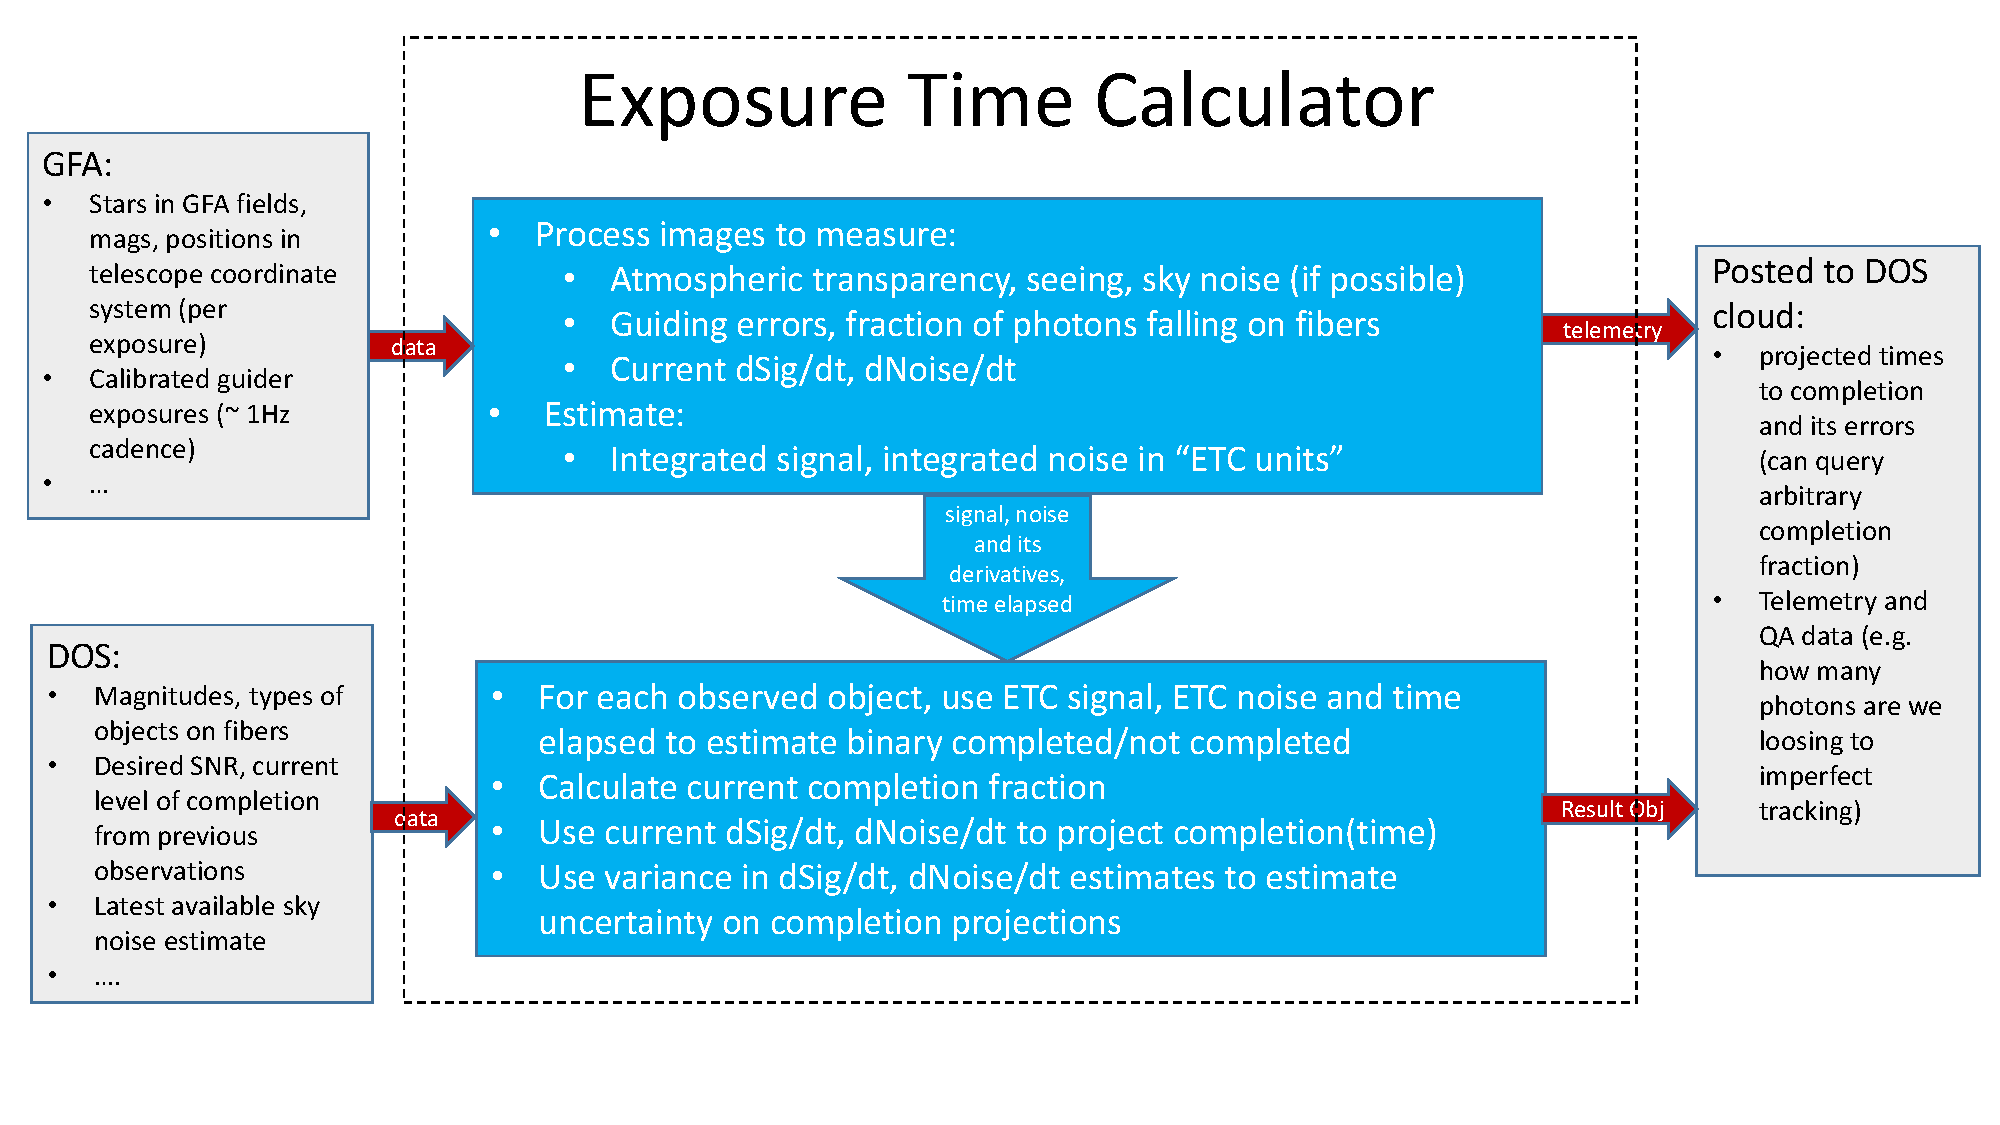
\includegraphics[width=\linewidth]{../Slides/SlideKlausMar15.pdf}
  \caption{Outline of the Exposure Time Calculator. Code implements area in dashed box.}
\label{fig:slide}
\end{figure}
Basic outline of the system is outlined in the Figure
\ref{fig:slide}. The problem is factorized into two sub-problems: i)
estimating the time derivatives of signal and noise as each time-stamp
given the GFA input in ``ETC units'' and ii) estimating the current
and projected completion of objects being observed given the history
of signal and noise derivatives.

\subsection{Estimating $d$Signal$/dt$ and $d$Sky$/dt$}
\label{sec:estim-dsign-dskydt}


The ``ETC units'' for signal and noise correspond to the number of
electrons being observed in a given passband for a star of a fiducial
magnitude in that passband.

For each guiding star, we can estimate the corresponding rate of
acquiring photons by lying down a synthethic aperture corresponding to
fiber size at the position where the star should have been, counting
photons in it and correcting for the background (sky+dark current):

\begin{equation}
  \left(\frac{d\mbox{Signal}}{dt}\right)_{\mbox{star\ } i} =
  \left[(\mbox {\#  photons in the synthethic aperture}) -
    \mbox{bias}\right] f_t f_{m,i} f_{s,i},
\end{equation}
where $\mbox{bias}$ is the average number of photons detected on the
same-sized apertures where no object resides, $f_t\sim 1+\epsilon$
corrects for the fact that GFA does not collect photons during its
readout, $f_m$ corrects for the fact that the guiding star is not
of a fiducial magnitude, ie. $f_m=10^{0.4\Delta M}$ and $f_s$ is a
correction for the fact the guide star might not be of a fiducial
spectral type. The relative error on this quantity is dominated by the shot
noise on the number of photons in the synthetic aperture. 
The total value of $d$Signal$/dt$ is then calculated as a weighed
averages of individual values.

The sky background is estimated as
\begin{equation}
  \left(\frac{d\mbox{Sky}}{dt}\right) =
  \left[(\mbox{bias}-(\mbox{dark current in the synthethic aperture})\right] f_t,
\end{equation}
The relative error on this measurement is given by the shot noise on
$\mbox{bias}$ number of electrons. If the dark current is too large,
the error on sky background might be unacceptably large.


\newcommand{\pr}{\textit{Possible refinements:}}

\pr
\begin{itemize}
\item Track guiding losses by repeating the measurement with a synthethic
  fiber stationed at actual star centroid rather than the nominal
  center
\item Track PSF losses by estimating the signal had the PSF been
  nominal rather than observed
\end{itemize}



\subsection{Estimating completion per object on the plate}
\label{sec:estim-compl-per}
For a given history of $d$Signal$/dt$ and $d$Sky$/dt$ we can calculate
the total Signal, Sky and time $t$.
For a given object $i$, the relative completion can be written as
\begin{equation}
  \mbox{completion}_i = \frac{(\mbox{Signal}) g_{m} g_{t}}
{\sqrt{(\mbox{Signal}) g_{m} g_{t}+(\mbox{Sky})g_{s} + g_{\rm
      dc}t+g_{\rm ro}}},
\end{equation}
where $g_{s,i}$ converts the signal in ETC units to a desired Signal
for a target object type depending on object type (LRG, ELG, QSO) at
fiducial magnitude for that object, $g_{m,i}=10^{-0.4 \Delta M}$
corrects for the fact that the targeted object is not of a fiducial
magnitude, $g_s$ converts the sky photons in ETC units to sky photons
at the desired passband for the particular object and $g_{\rm dc,i}$
is the spectrographs CCDs dark current given and $g_{\rm dc,i}$ and
$g_{\rm ro}$ is the spectrograph readout noise. Note that all $g$
parameters depends on the target object's type and possibly red-shift
with $g_m$ additionally depending on its magnitude. Note also that
$g_s$ can be rescales so that completion$_i=1$, when the a desired SNR
has been reached. All the values of $g$ are best calibrated using
commissioning runs and can be refined further as time progresses.

\subsection{Estimating the current observation's completion and
  projected time to completion.}
\label{sec:estim-curr-observ}
From the beginning of the observations, we can tabulate past
$d$Signal$/dt$, $d$Sky$/dt$ as described in Section
\ref{sec:estim-dsign-dskydt} and then for each observed object,
estimate its completion as described in the Section
\ref{sec:estim-compl-per}. The fraction of object that are completed
is the current completion fraction.

Using the latest estimated of $d$Signal$/dt$ and $d$Sky$/dt$, we can
also make our best guess of the future Signal and Sky values as a
function of time and feed these into the completion code. We call a
plate complete when the completion fraction is $100$\%.  Using the
variance of the past measurements of $d$Signal$/dt$ and $d$Sky/$dt$
(correctly accounting for the error in those measurements -- the idea
is to measure intrinsic variability of the conditions as the
observation progresses) we can project future
``histories'' that have 1 sigma higher signal and 1 sigma lower noise
and feed those to find the lower limit on the projected time to
completion. Ditto for 1 sigma worse projected conditions to find the
upper limit on the projected conditions. The idea is to give a rough
estimate of the error on the projected time to completion. 

\pr
\begin{itemize}
\item Refined error on the projected time to conditions by
  bootstrapping over possible future histories
\item Better estimate of losses due to tracking, PSF, sky to give
  feedback for possible improvements of the system
\end{itemize}


\section{Estimating viability}

See Kevin Reil's doc. To be written.






\section{Code Objects}

Code sits under \texttt{desihub} as \texttt{desietc}. 

The basic layout
is as follows:

\begin{itemize}
\item \texttt{etc.py} is the basic interface to the outer world and
  implements logic described in \ref{sec:estim-curr-observ}.
\item \texttt{GuiderPackProcessor.py} implements logic described in 
\ref{sec:estim-dsign-dskydt}
\item \texttt{TargetsProcessor.py} implements logic described in
  \ref{sec:estim-compl-per}.
\item \texttt{ETCGuidePack.py} is a data holding object that contains
  calibrated GFA images
\item \texttt{ETCTargets.py} is a data holding object that contains
  the description of the objects on the plate
\item \texttt{ETCResults.py} is a data holding object that contains
  the results of the ETC processing. It knows the time to completion
  and the error on this.
\end{itemize}


\end{document}
